% -*- LaTeX -*-
% -*- coding: utf-8 -*-
%
% michael a.g. aïvázis <michael.aivazis@para-sim.com>
% (c) 2003-2017 all rights reserved
%

\section{components}
\subsection{basics}

\begin{frame}
%
  \frametitle{Components and protocols}
%
  \begin{itemize}
%
    \item a design pattern that enables the assembly of applications out of interchangeable
      parts, under the control of the {\em end user}
      \begin{itemize}
      \item {\em protocols} are abstract specifications of application requirements
      \item {\em components} are concrete implementations that satisfy requirements
      \end{itemize}
%
    \item inversion of control:
      \begin{itemize}
      \item the binding of implementations to specifications happens at runtime, under the
        control of the end user
      \end{itemize}
%
    \item the user
      \begin{itemize}
      \item controls the application state through configuration files, the user interface, the
        command line
      \item specifies components using simple URIs
      \end{itemize}
%
    \item the goal is to isolate contributors from each other as much as possible, and provide
      a coherent and usable strategy for composing non-trivial applications
%
  \end{itemize}
%
\end{frame}

%-----------------------------------
\begin{frame}
%
  \frametitle{Components}
  %
  \begin{center}
    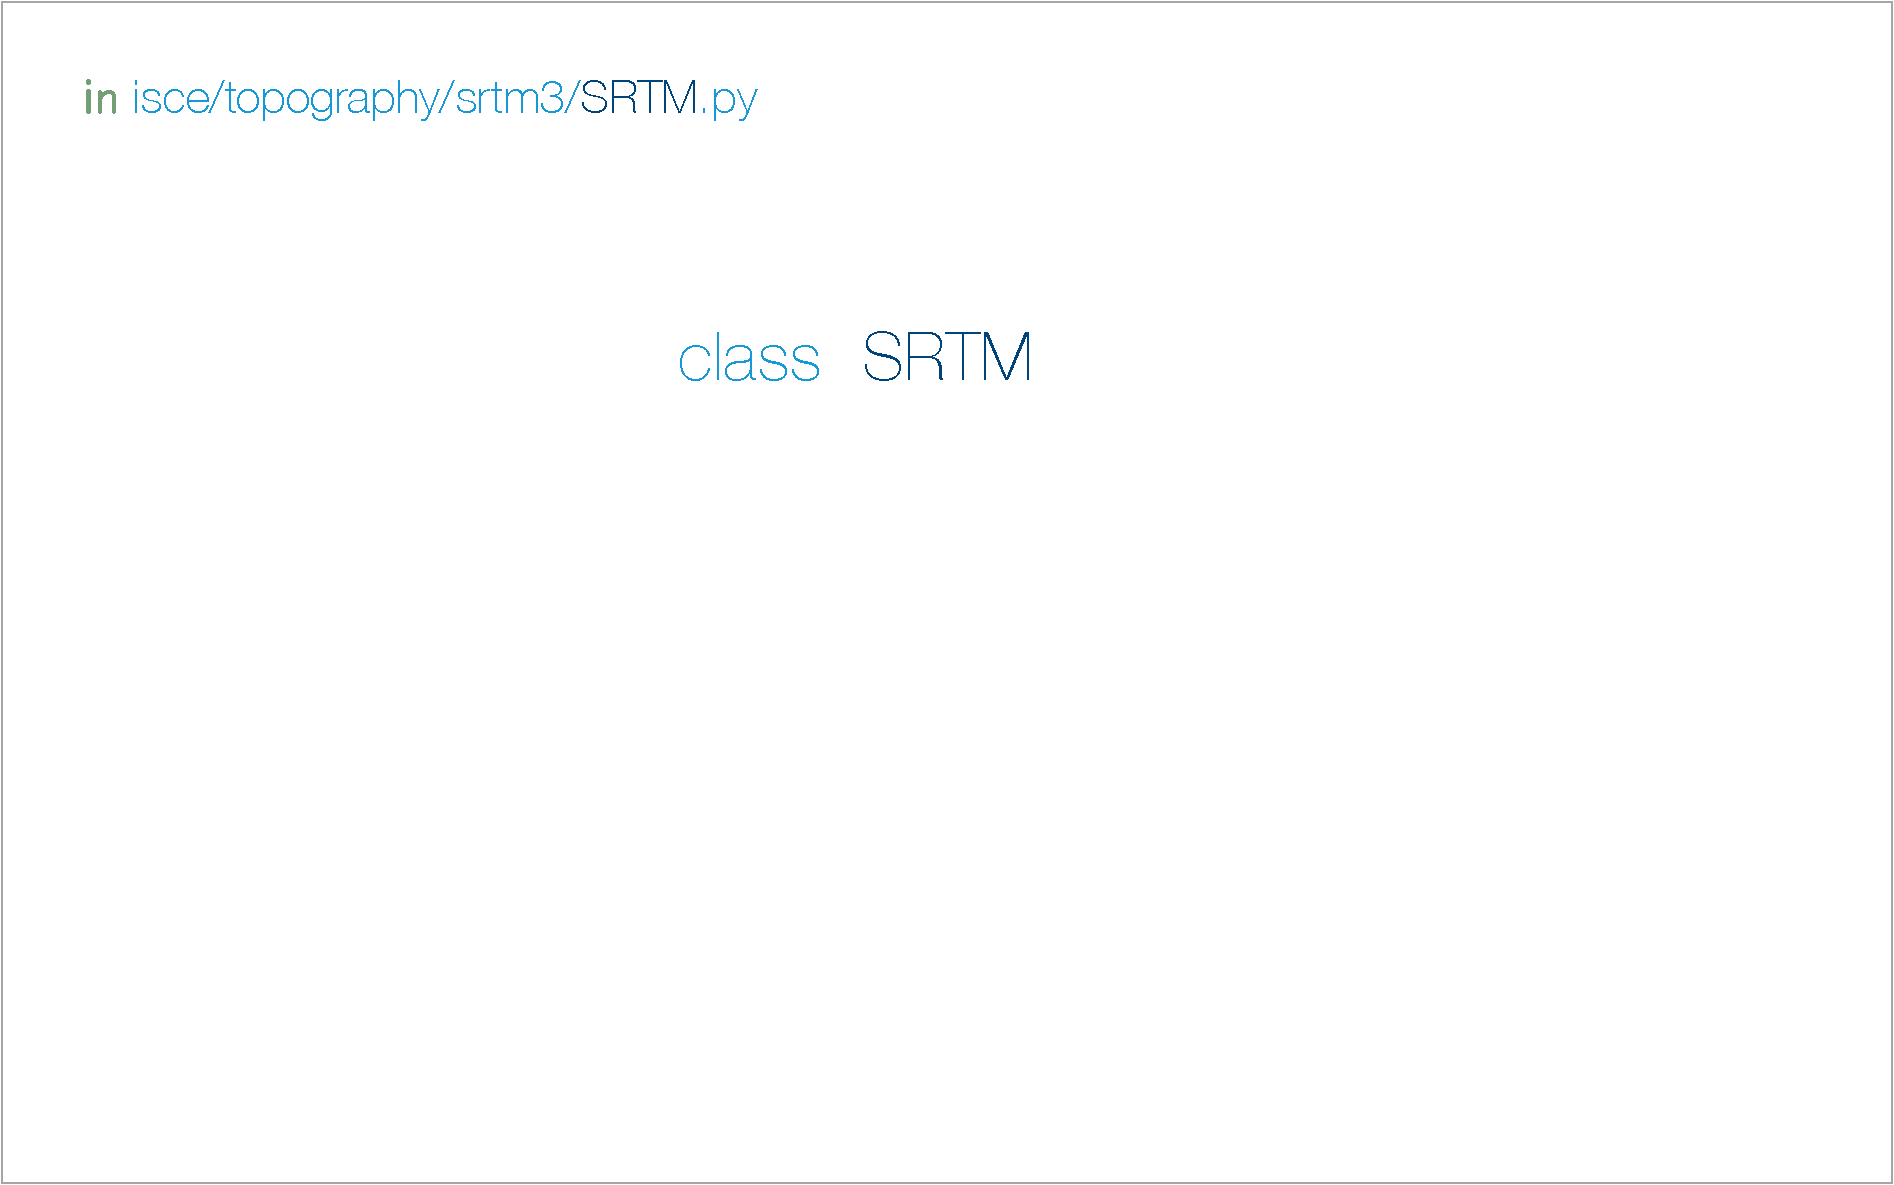
\includegraphics[width=1.0\textwidth]{component-package}
  \end{center}
  %
\end{frame}

%-----------------------------------
\begin{frame}
%
  \frametitle{Components}
  %
  \begin{center}
    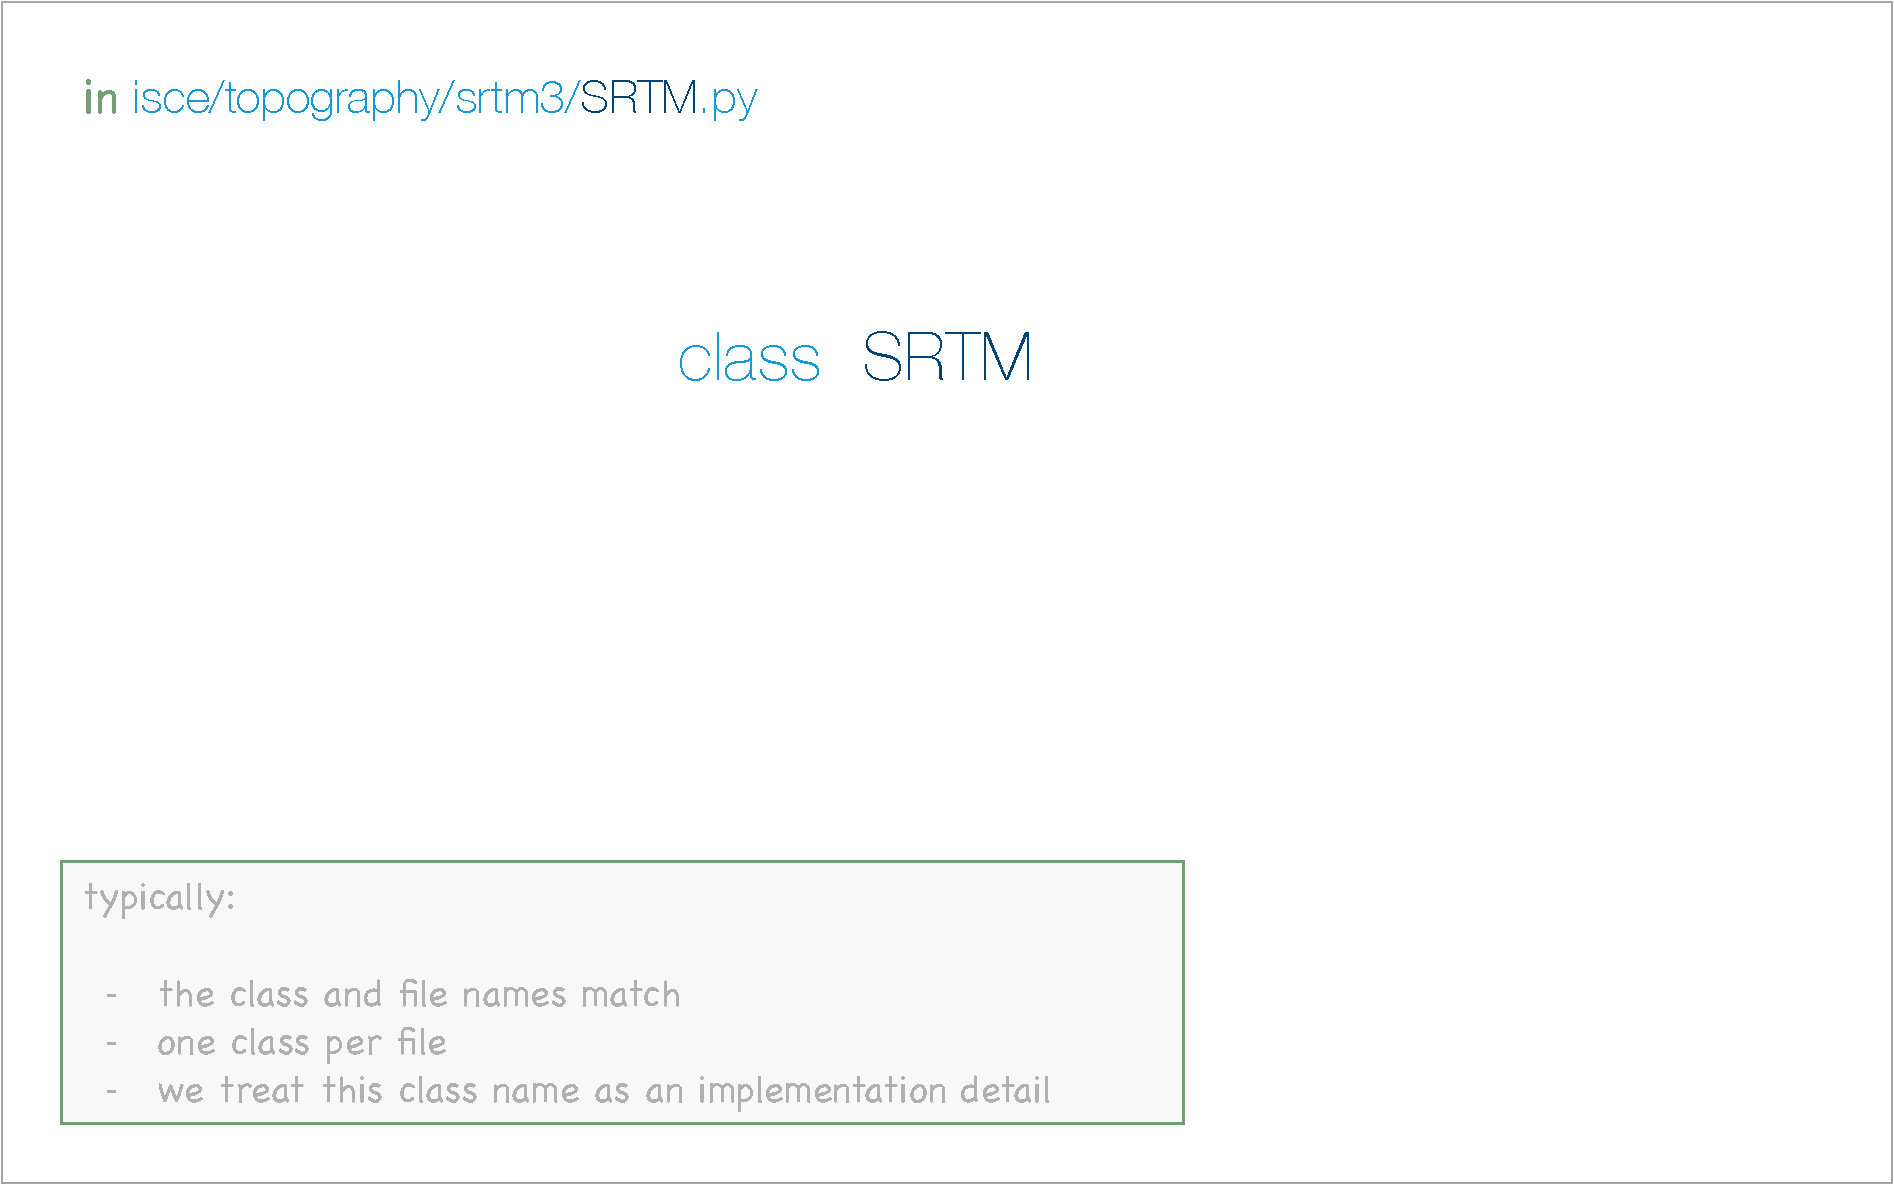
\includegraphics[width=1.0\textwidth]{component-package-explained}
  \end{center}
  %
\end{frame}

%-----------------------------------
\begin{frame}
%
  \frametitle{Components}
  %
  \begin{center}
    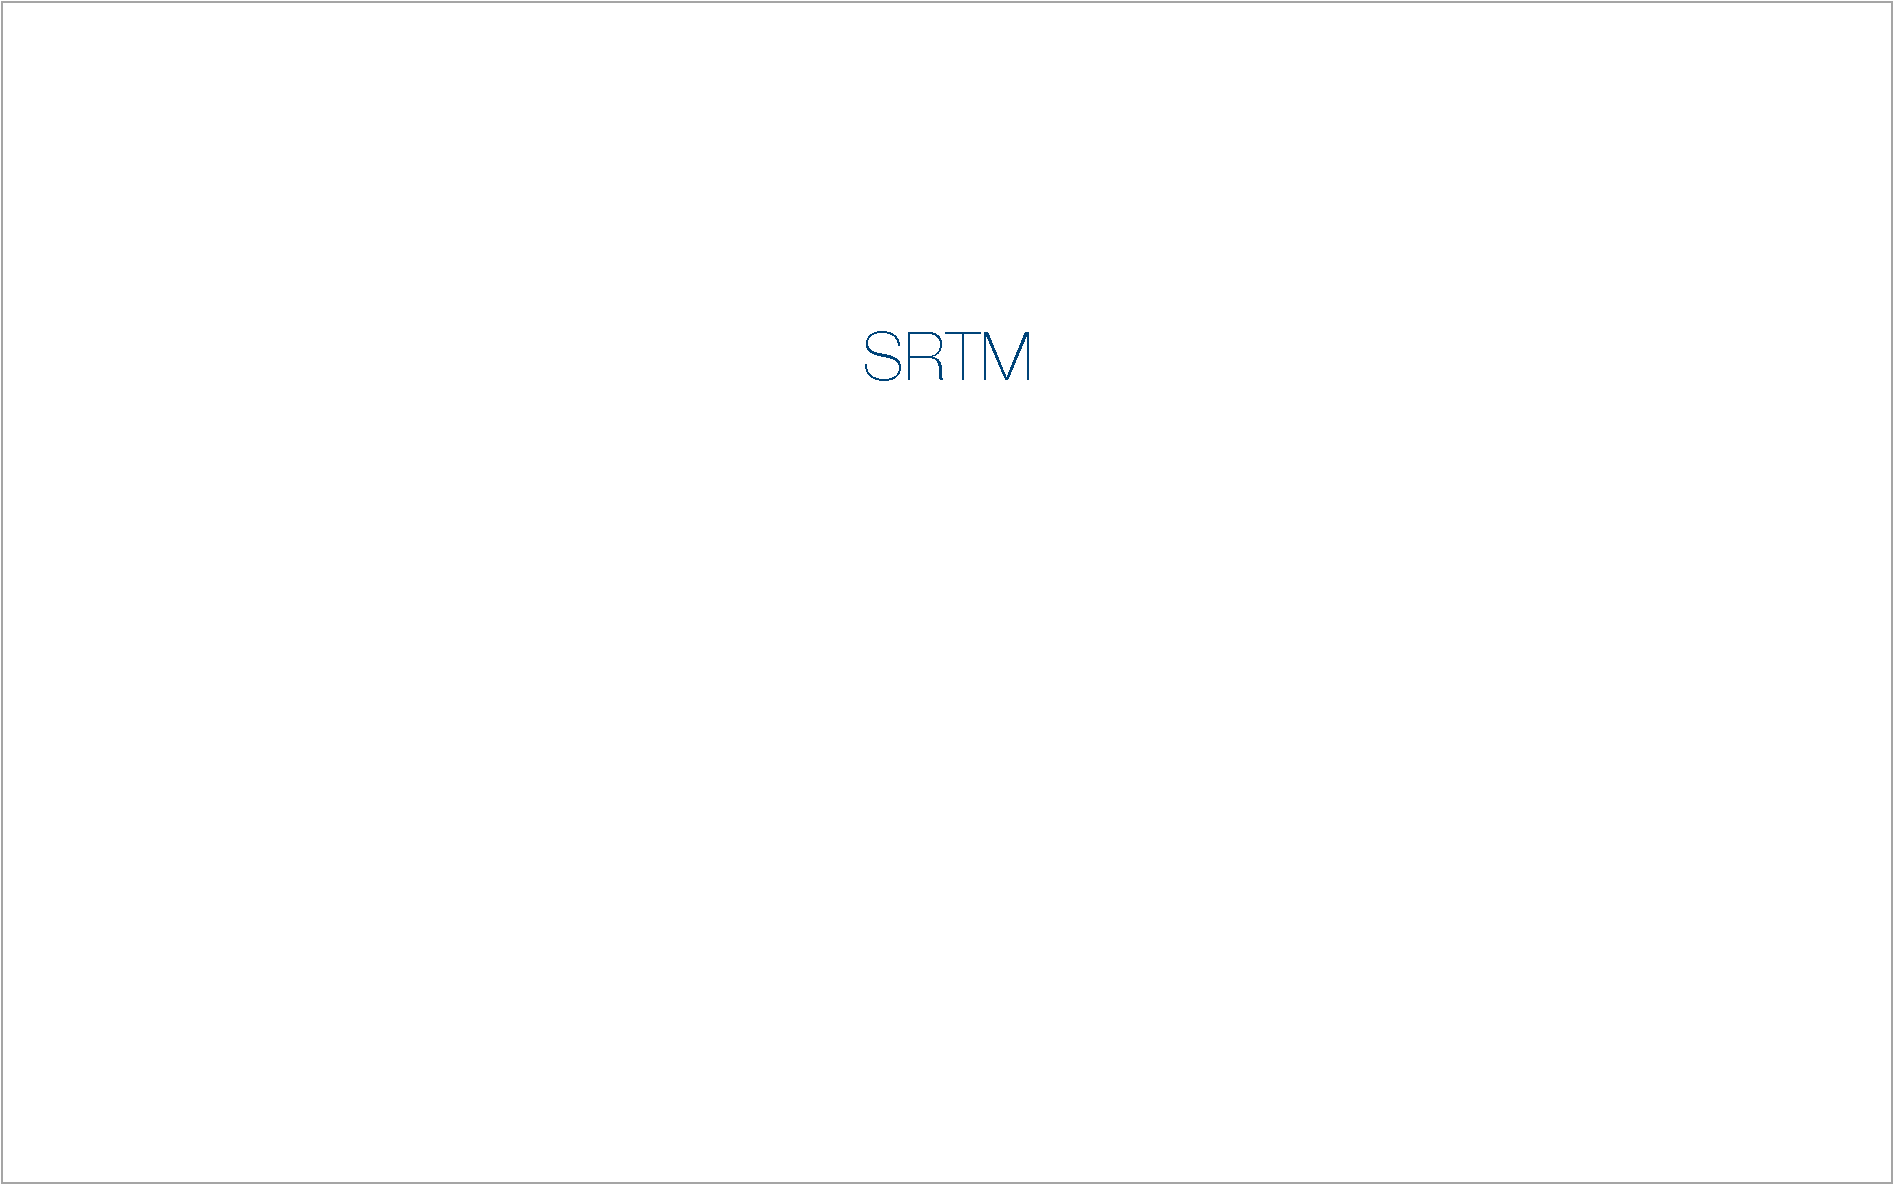
\includegraphics[width=1.0\textwidth]{component-base}
  \end{center}
  %
\end{frame}

%-----------------------------------
\begin{frame}
%
  \frametitle{Components}
  %
  \begin{center}
    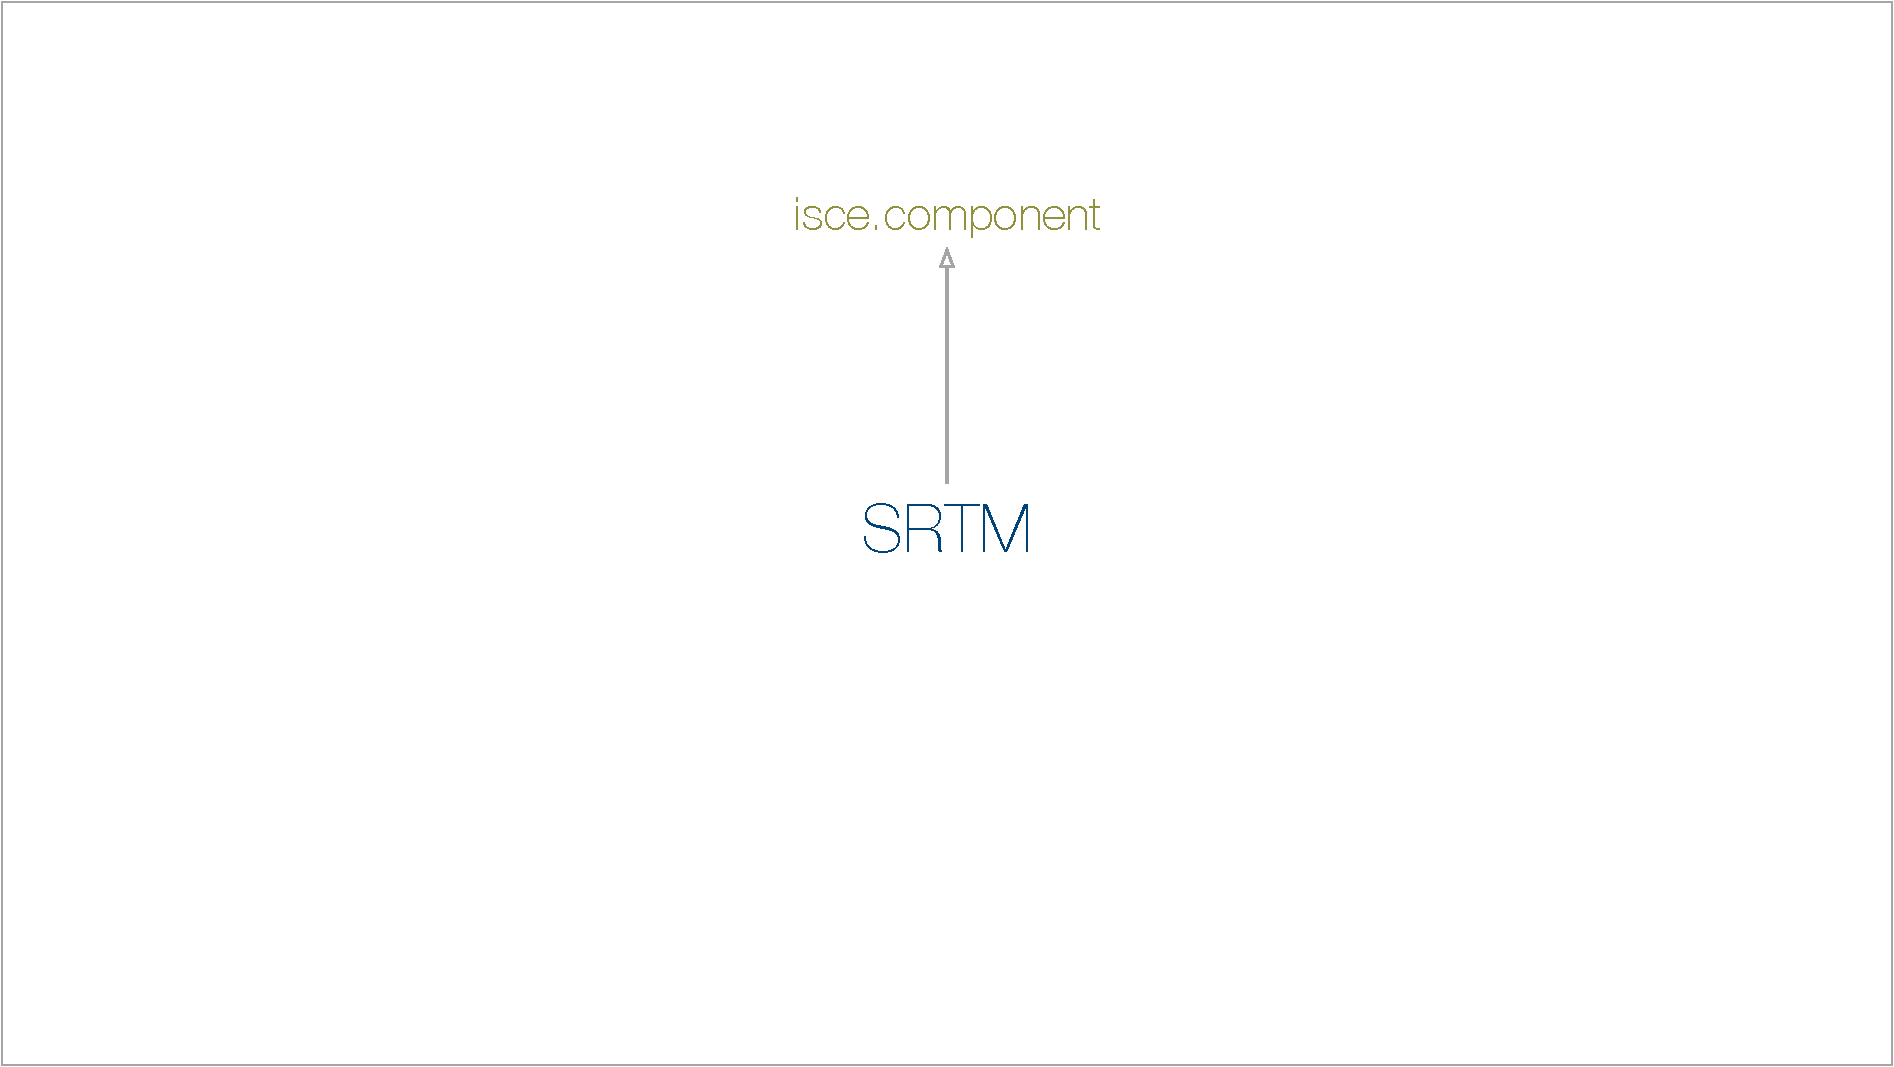
\includegraphics[width=1.0\textwidth]{component-inheritance}
  \end{center}
  %
\end{frame}

% --------------------------------------
% components:
\begin{frame}
%
  \frametitle{Components}
%
  \begin{itemize}
%
  \item informally, \emph{classes} are software specifications that establish a relationship
    between \emph{state} and \emph{behavior}
    \begin{itemize}
    \item we have syntax that allows us to specify these very close to each other
    \end{itemize}
%
  \item \emph{instances} are containers of state; there are special rules
    \begin{itemize}
    \item that grant access to this state
    \item allow you to call functions that get easy access to this state
    \end{itemize}
%
  \item \emph{components} are classes that specifically grant access to some of their state to
    the end user
    \begin{itemize}
    \item the public data are the \emph{properties} of the component
    \end{itemize}
%
  \item rule 1: components have properties
%
  \end{itemize}
%
\end{frame}

%-----------------------------------
\begin{frame}
%
  \frametitle{Components}
  %
  \begin{center}
    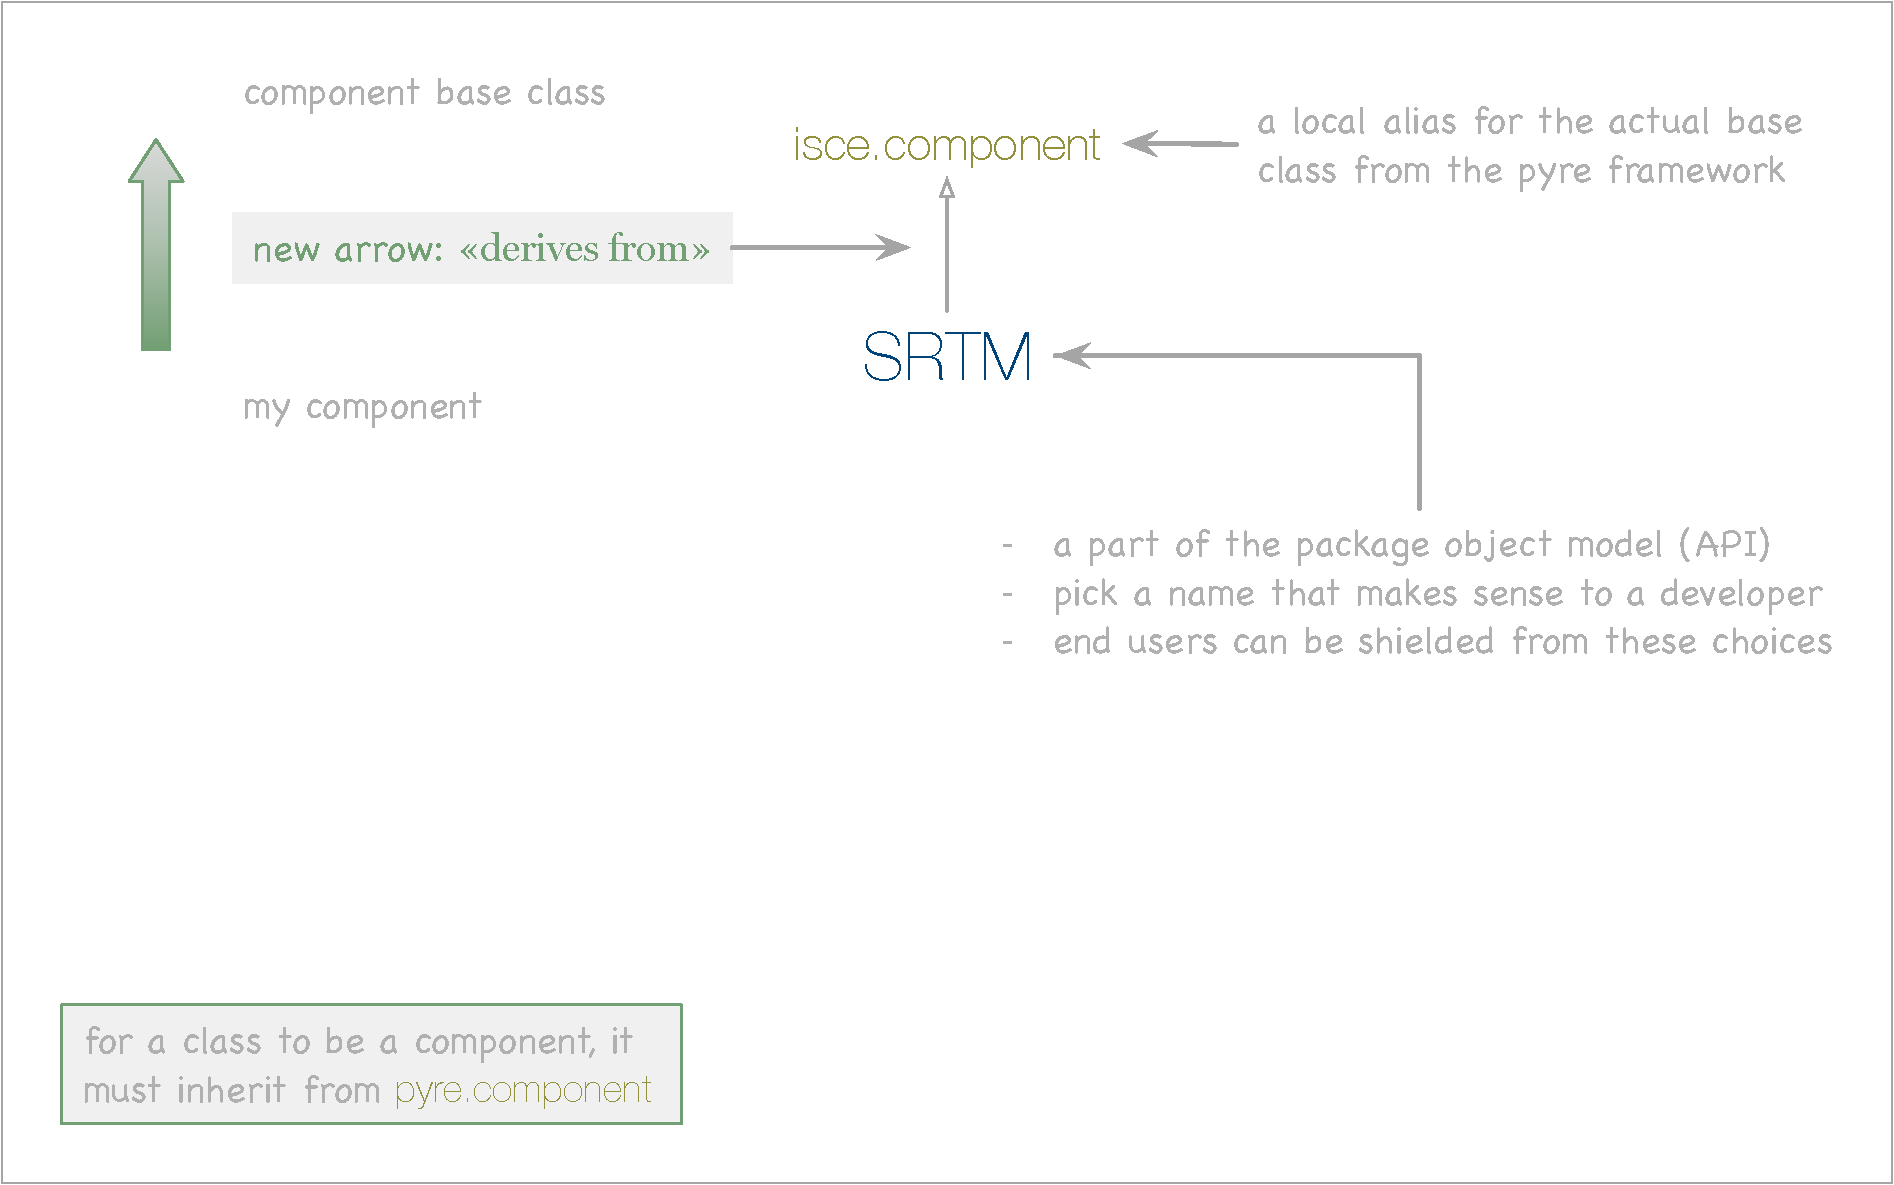
\includegraphics[width=1.0\textwidth]{component-inheritance-explained}
  \end{center}
  %
\end{frame}

%-----------------------------------
\begin{frame}
%
  \frametitle{Components}
  %
  \begin{center}
    
\includegraphics[width=1.0\textwidth]{component-family}
  \end{center}
  %
\end{frame}

%-----------------------------------
\begin{frame}
%
  \frametitle{Components}
  %
  \begin{center}
    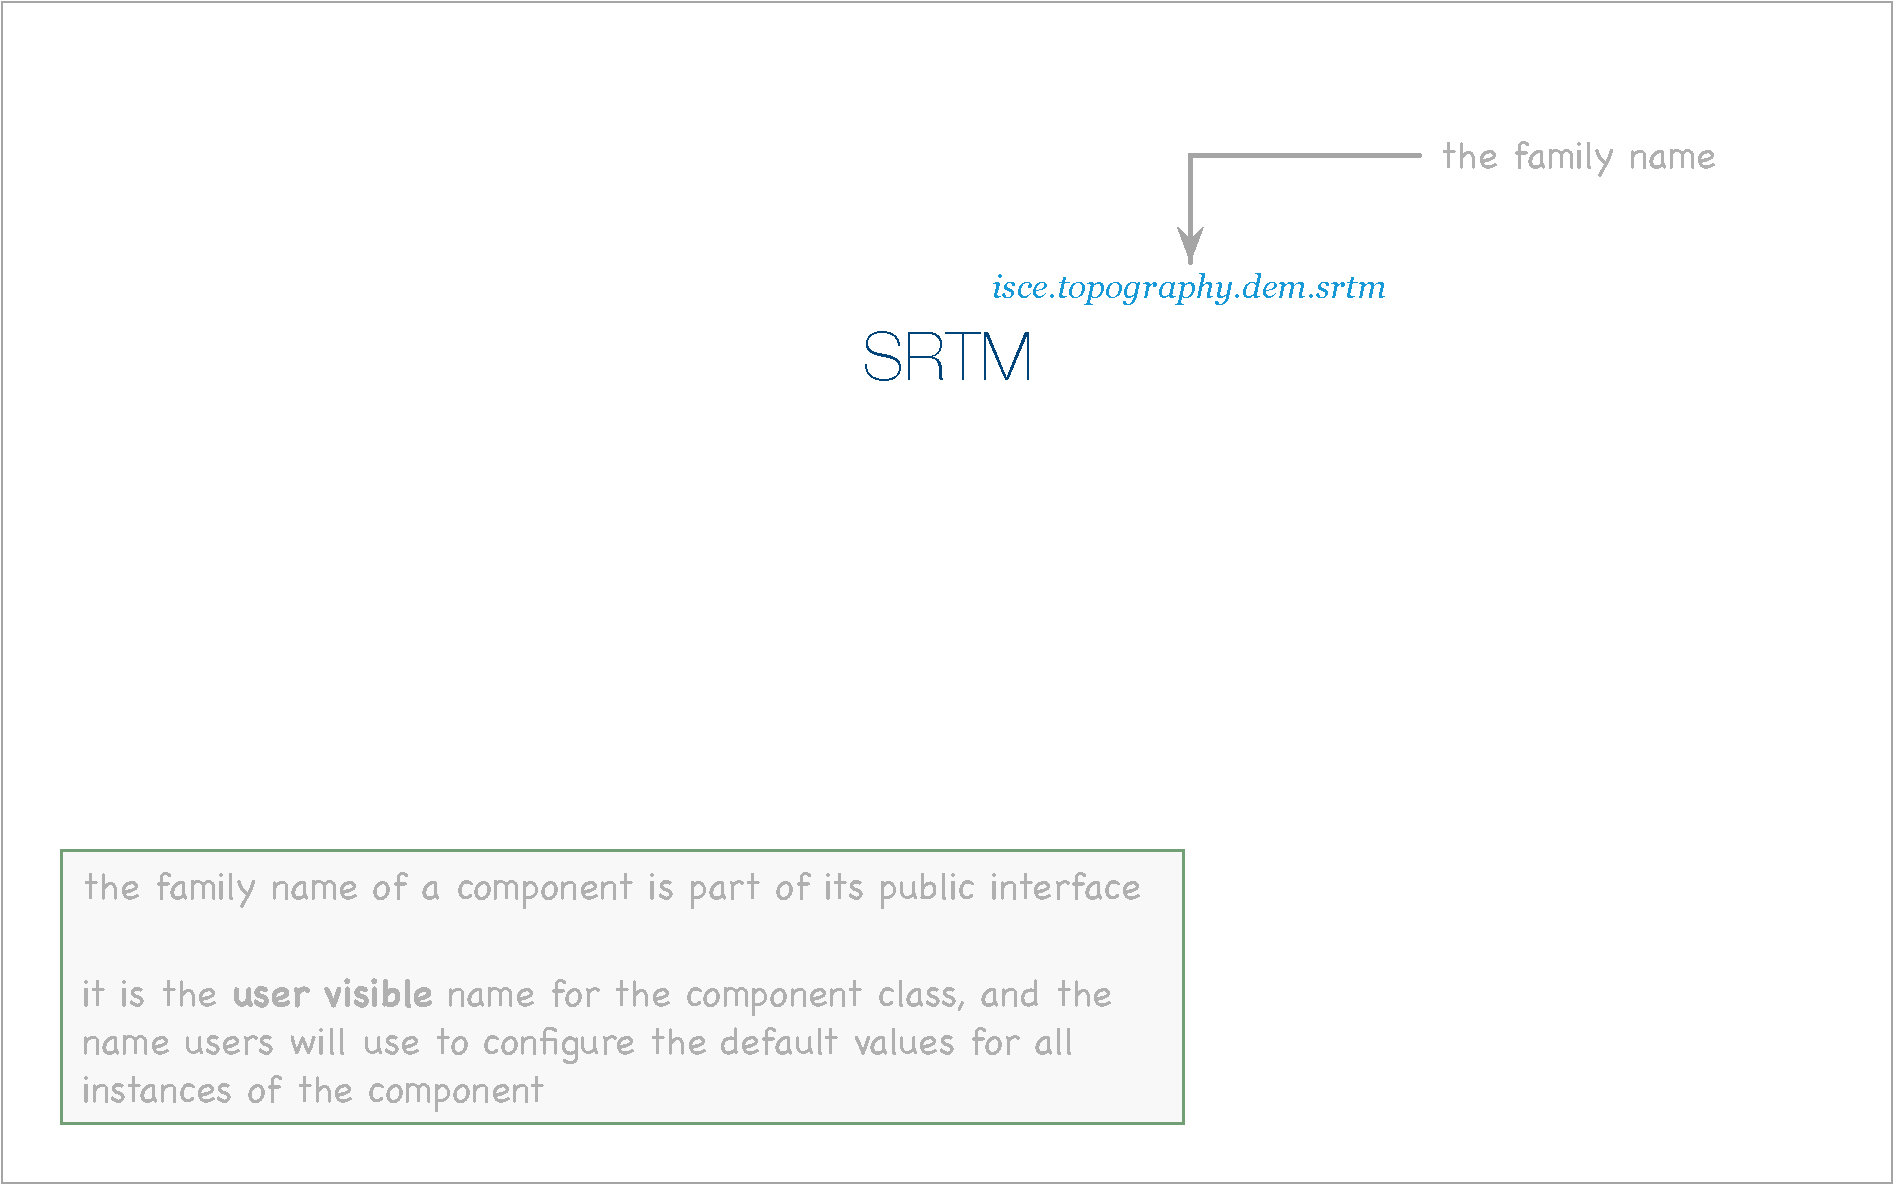
\includegraphics[width=1.0\textwidth]{component-family-explained}
  \end{center}
  %
\end{frame}

%-----------------------------------
\begin{frame}
%
  \frametitle{Components}
  %
  \begin{center}
    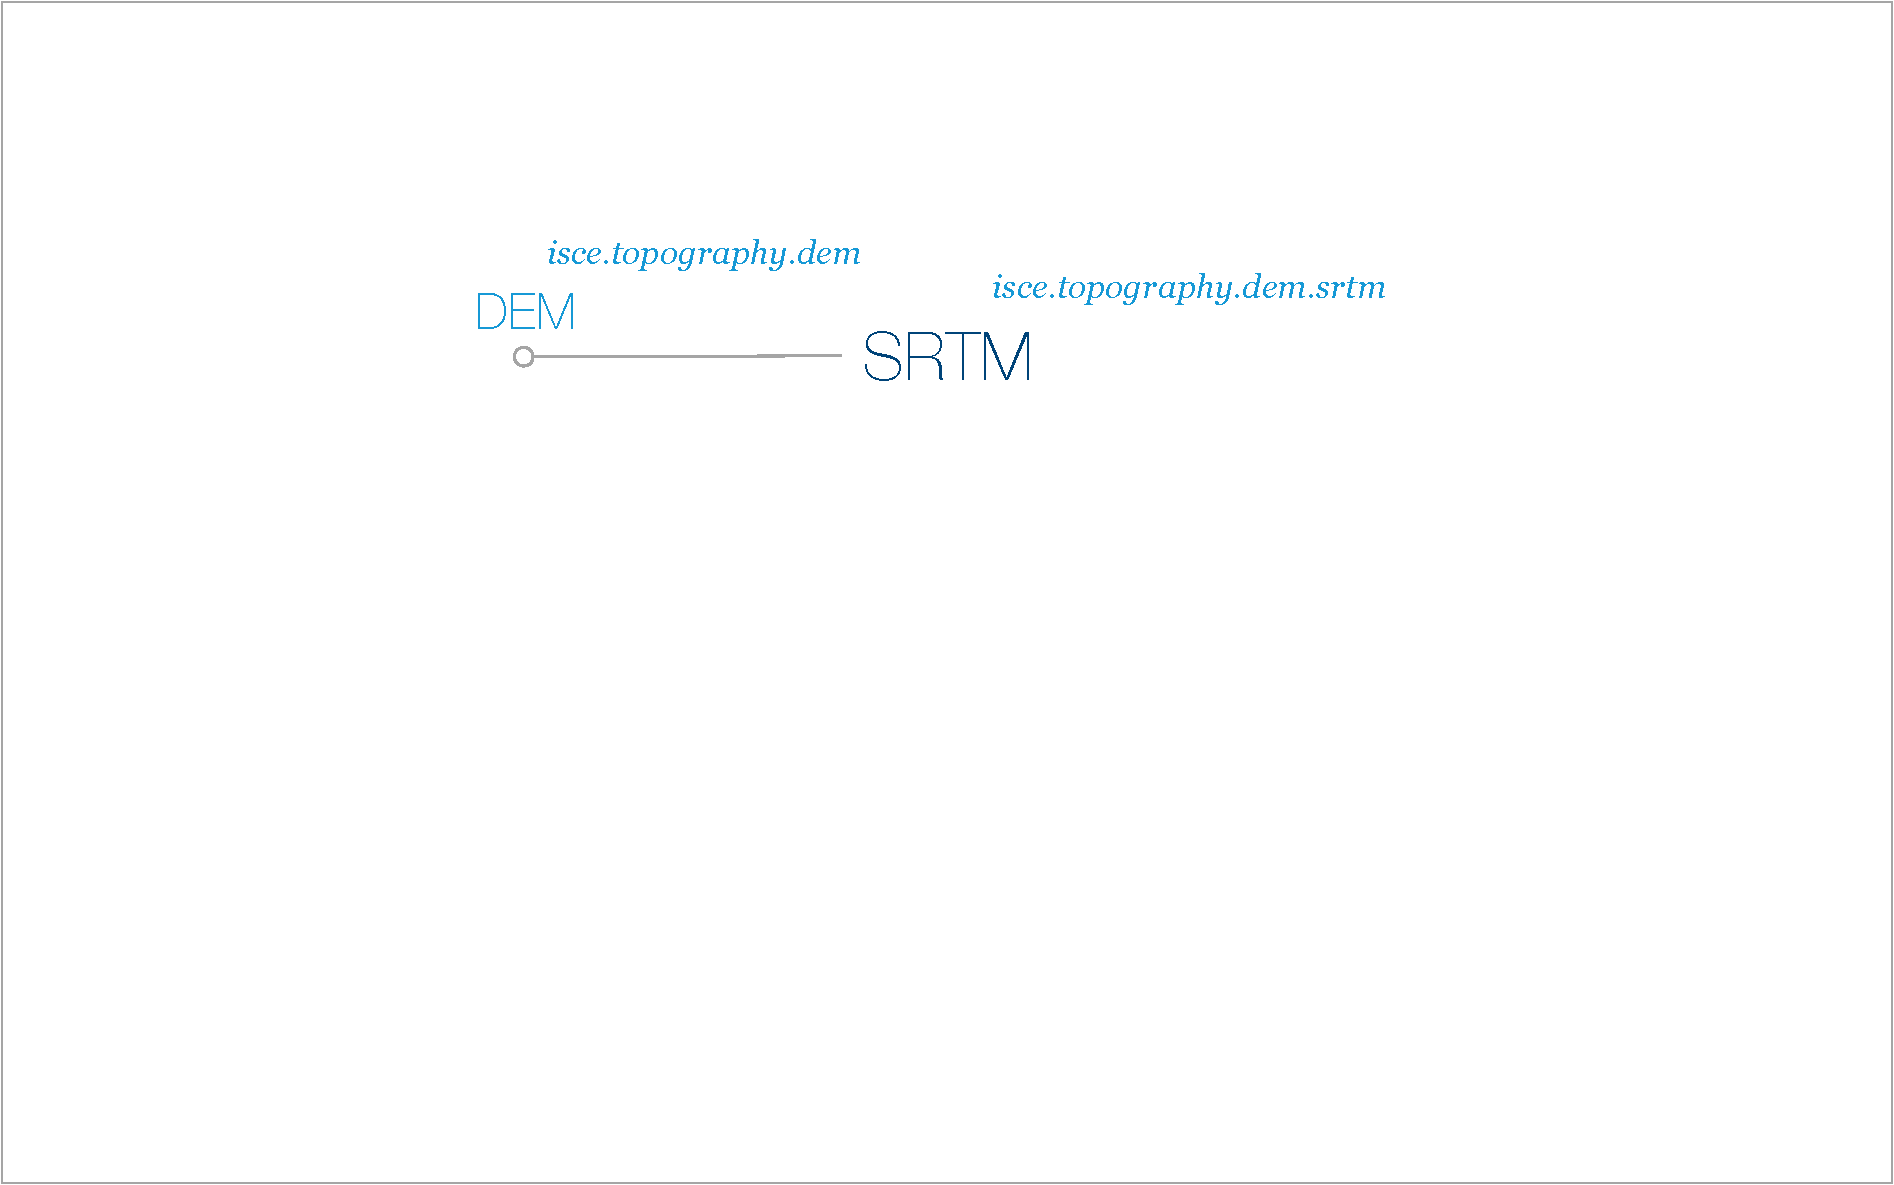
\includegraphics[width=1.0\textwidth]{component-implements}
  \end{center}
  %
\end{frame}

%-----------------------------------
\begin{frame}
%
  \frametitle{Components}
  %
  \begin{center}
    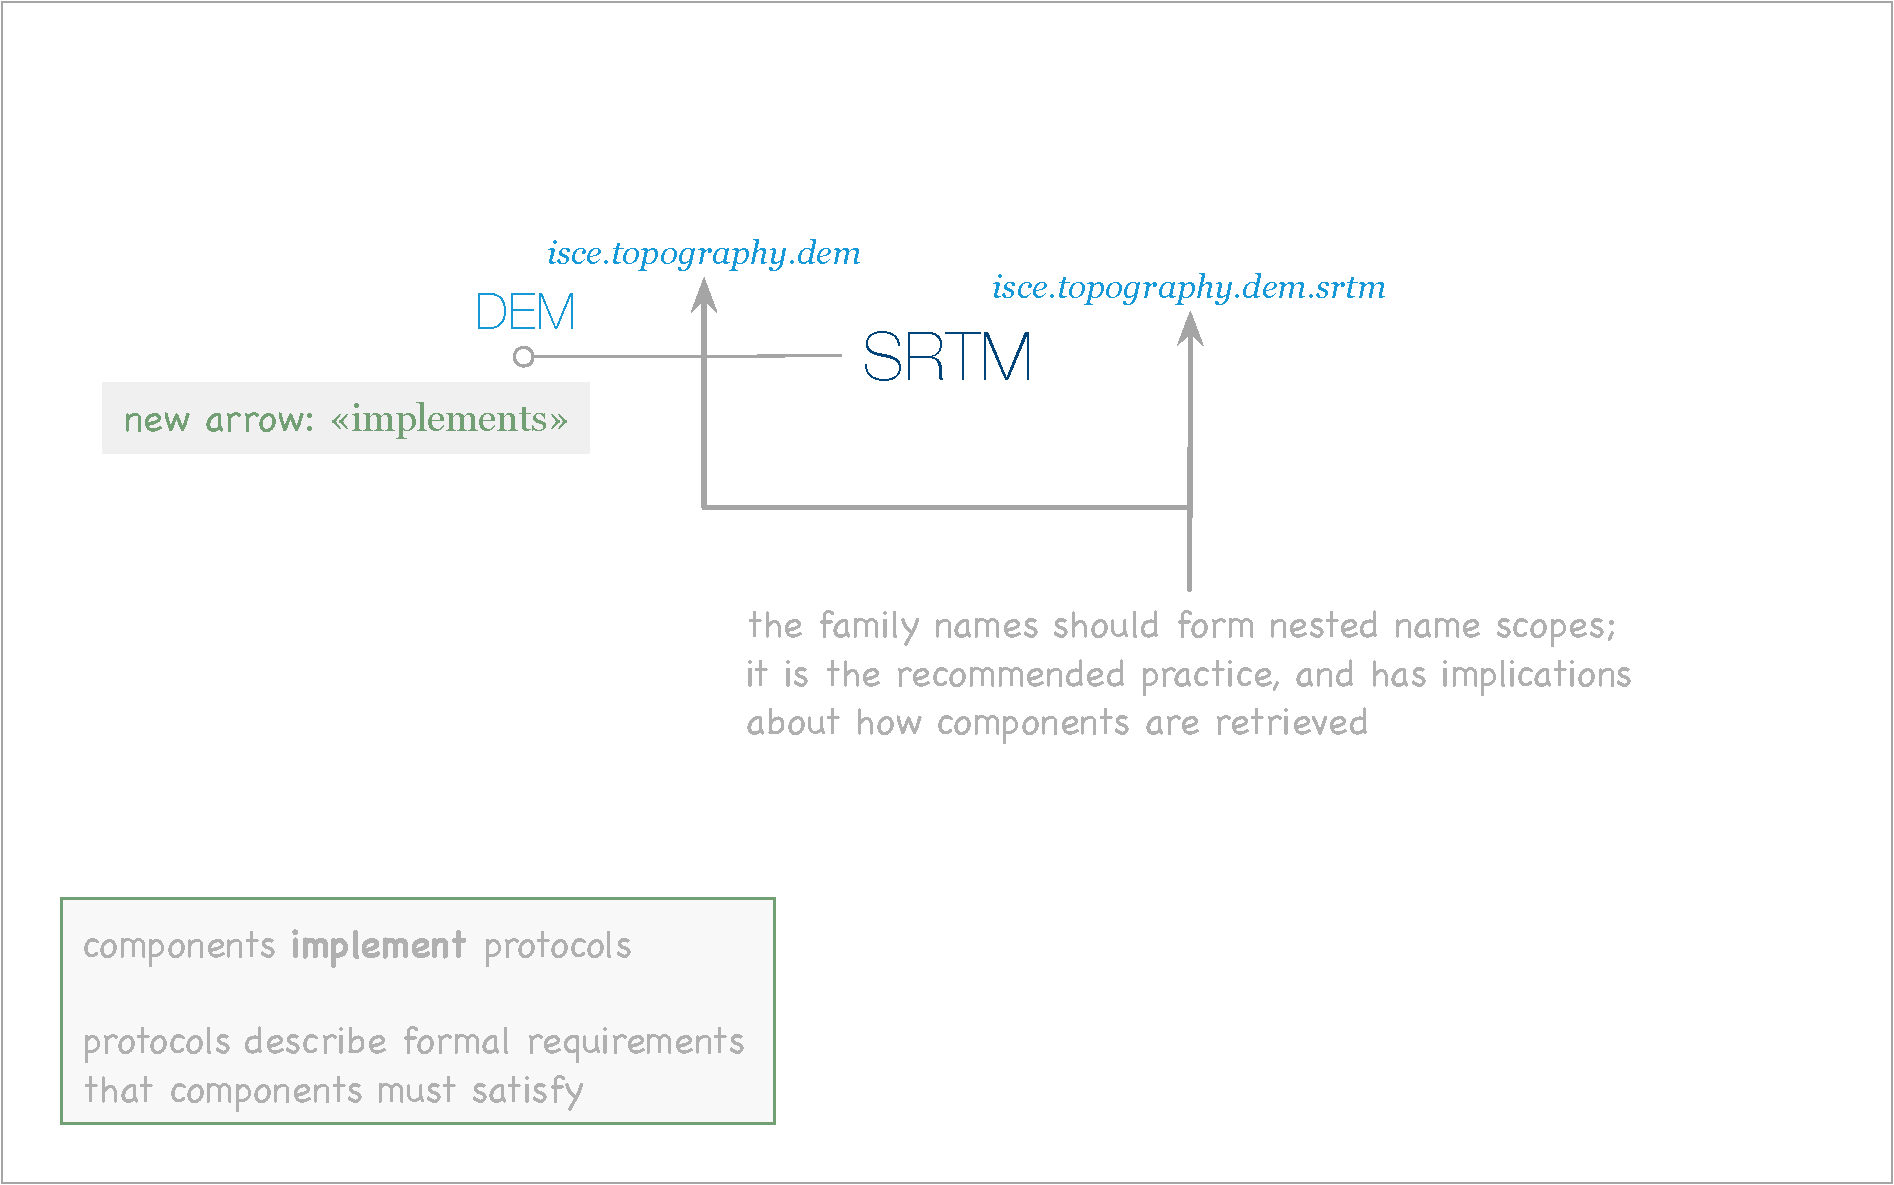
\includegraphics[width=1.0\textwidth]{component-implements-explained}
  \end{center}
  %
\end{frame}

% --------------------------------------
% recap
\begin{frame}
%
  \frametitle{Recap: what we know so far}
%
  \begin{itemize}
%
  \item \pyre\ components are evolved python objects
    \begin{itemize}
    \item the factories have family names, the instances have names
    \item these names are unique strings in hierarchical namespaces delimited by periods
    \item collections of components form packages \emph{implicitly}, based on the topmost level
      in their namespace
    \end{itemize}
%
  \item components have properties that are under the control of the \emph{user}
    \begin{itemize}
    \item they look and behave like regular attributes
    \item they are \emph{typed} to enable conversions from strings
    \item they have default values and other metadata
    \end{itemize}
%
  \item configuration is partly about assigning values to component properties
    \begin{itemize}
    \item a requirement for supporting user interfaces
    \item intuitive syntax for the command line
    \item simple configuration files inspired by the Microsoft Windows \identifier{.ini} format
    \end{itemize}
%
  \item configuration is automatically handled by the framework and requires no explicit
    involvement on the part of the component author
%
  \end{itemize}
%
\end{frame}

% --------------------------------------
% properties
\begin{frame}
%
  \frametitle{Properties}
%
  \vskip -2ex
  \begin{itemize}
%
  \item properties make sense for both classes and instances
    \begin{itemize}
    \item the class holds the default value that gets used in case the component instance does
      not have explicit configuration
    \item each instance gets its own private value when it gets configured
    \item identical to regular python attributes
    \end{itemize}
%
  \item there is support for
    \begin{itemize}
    \item simple types: \function{bool}, \function{int}, \function{float}, \function{str}
    \item containers: \function{tuple}, \function{array}
    \item higher level: \function{date}, \function{time}, \function{inputfile},
      \function{outputfile}, \function{inet}
    \item units: \function{dimensional}
    \item easy enough to implement your own; the requirements are very simple
    \end{itemize}
%
  \item metadata:
    \begin{itemize}
    \item \identifier{doc}: a simple and short documentation string
    \item \identifier{default}: the default value, in case the user doesn't supply one
    \item \identifier{converters}: a chain of preprocessors of the string representation
    \item \identifier{normalizers}: a chain of post-processors of the converted value
    \item \identifier{validators}: a tuple of predicates that get called to ensure the property
      value satisfies the specified constraints
    \item you can add your own; the framework passes them through to your component
    \end{itemize}
%
  \end{itemize}
%
\end{frame}

% --------------------------------------
% units
\begin{frame}[fragile]
%
  \frametitle{Units}
%
  \vskip -2ex
  \begin{itemize}
%
  \item \function{dimensional} properties have units
%
  \item the low level support is in \package{pyre.units}
    \begin{itemize}
    \item full support for all SI base and derived units
    \item all common abbreviations and names from alternative systems of units
    \item correct arithmetic; proper handling of functions from \package{math}
    \end{itemize}
%
    \begin{ipython}{}
from math import cos
from pyre.units.SI import meter, second, radian

A = 2.5 * meter
t = 1.5 * second
ω = 4.2 * radian/second

x = A * cos(ω * t)
    \end{ipython}
%
    if the units in the argument to \function{cos} do not cancel, leaving a pure
    \keyword{float} behind, an exception is raised; \identifier{x} has dimensions of meters
%
  \end{itemize}
%
\end{frame}

%%% Local Variables:
%%% mode: latex
%%% TeX-master: "../pyre"
%%% End:

% end of file
